\documentclass[compress]{beamer}
%\documentclass[compress, handout]{beamer}

% To create a handout: uncomment below and add handout as an option
% for documentclass
%\usepackage{pgfpages}
%\pgfpagesuselayout{4 on 1}[a4paper, landscape, border shrink=5mm]

% not all of the packages below will be needed
\usepackage[T1]{fontenc}
\usepackage[ngerman]{babel}
\usepackage[utf8]{inputenc}
\usepackage{units}
\usepackage{amsmath}
\usepackage{amsfonts}
\usepackage[amssymb]{SIunits}
\usepackage{amssymb}
\usepackage{microtype}
\usepackage{bbm}
\usepackage{booktabs}
\usepackage{simpleMath}

\usepackage[TOC]{style} % add option 'TOC' if you want an Outline before every section

\usepackage{graphicx}
%\graphicspath{{Figures/}} % uncomment to use a standard graphics location


\title{Chaos}
\titlegraphic{
\includegraphics[width=0.9\textwidth]{Figures/NAT_SIGN_druck_SW}}
\subtitle{Eine (sehr) kurze Einführung} % (optional)
\author{Alexander Eberspächer}

\date{19. November 2012} % \today ?
\subject{Chaos - eine kurze Einführung}


\begin{document}

\begin{frame} % title
  \titlepage
  \thispagestyle{empty}
\end{frame}

\begin{frame}{Outline} % first Outline
  \tableofcontents
\end{frame}

% Input your presentation's contents here
\section{Einführung}

\subsection{Einführung}

\begin{frame}{Chaos?}

  \begin{alertbbox}{Chaos}
    \emph{``Durcheinander, totale Unordnung''}\\[0.5ex]
    \scriptsize{\hspace{0.5ex} -- Reclam, ``Kleines Fremdwörterbuch''}
  \end{alertbbox}

  \pause

  Für unsere Zwecke:

  \begin{bbox}{Chaos bedeutet...}
    \begin{itemize}
    \item komplizierte Dynamik
    \item mit sensitiver Abhängigkeit von Anfangsbedingungen
    \end{itemize}
  \end{bbox}

  \pause

  Dennoch folgt chaotische Dynamik \alert{deterministischen} Gesetzen!
\end{frame}


\begin{frame}{Unser erstes System: das getriebene Pendel}

  \begin{columns}
    \column{0.45\textwidth}

    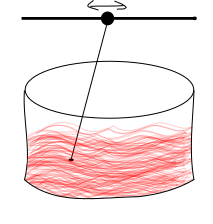
\includegraphics[width=1.05\linewidth]{Figures/Pendel.pdf}

    \column{0.55\textwidth}

    Im Ruhesystem der Aufhängung:

    \begin{itemize}
    \item rückstellende Kraft $F_1 = -mg\sin(\phi)$
    \item Kraft durch bewegte Aufhängung $F_2 = F_\mathrm{ext}$
    \item Reibung $F_3 = -2\gamma\dot{\phi}$
    \end{itemize}
    \pause
    Für harmonische treibende Kraft $F_\mathrm{ext} = A\sin(\omega_\mathrm{d}t)$:\\[-2.5ex]
    \[  m l \ddot{\phi} = -mg\sin(\phi) - 2\gamma\dot{\phi} + A\sin(\omega_\mathrm{d}t)\]
  \end{columns}
  \pause
  \vspace{1.0ex}
  Antrieb\&Dämpfung: \emph{dissipatives System}\\
  Kraft $\propto \sin(\phi)$: \alert{nichtlineares System}
\end{frame}


\begin{frame}{Pendel: kein Antrieb}

  \begin{columns}

    \column{0.5\textwidth}
    Setze $m=l=g=1$, $\gamma =0.25$, $\omega_\mathrm{d}=2/3$.\\[0.5ex]

    Zunächst $A=0$:\\[1.5ex]

    \includegraphics[width=\linewidth]{Figures/PendelA0-Zeit.pdf}

    \column{0.5\textwidth}

    \only<2,3>{

      \only<2>{DGL \emph{2. Ordnung}: Dynamik durch $\phi$ \emph{und} $\dot{\phi}$ beschrieben}

      \begin{alertbbox}{$\leadsto$ Phasenportrait}
        $\dot{\phi} = \dot{\phi}(\phi(t))$; $t$ parametrisiert die Kurve
      \end{alertbbox}
      \only<3>{
        \includegraphics[width=\linewidth]{Figures/PendelA0-Phase.pdf}}
    }

  \end{columns}

  \only<3>{$\vec\xi = (\phi, \dot{\phi}) = (0,0)$ ist ein \emph{Punkt\alert{attraktor}}}

\end{frame}


\begin{frame}{Pendel: etwas Antrieb}

  \begin{columns}

    \column{0.5\textwidth}
    Jetzt: $A=0.5$\\[1.5ex]

    \includegraphics[width=\linewidth]{Figures/PendelA05-Zeit.pdf}

    \column{0.5\textwidth}

    \only<2>{
      Phasenportrait:\\[1.5ex]
      \includegraphics[width=\linewidth]{Figures/PendelA05-Phase.pdf}
    }

  \end{columns}

  \only<2>{Die Lösungen konvergieren gegen einen \alert{Grenzzyklus} oder $1d$-Attrakor}

\end{frame}


\begin{frame}{Pendel: \emph{Mehr Power!}}

  \begin{center}
    \includegraphics[width=0.7\textwidth]{Figures/power.jpg}
  \end{center}
  \vspace{4ex}\scriptsize{Bild von http://www.mobilemag.com}
\end{frame}


\begin{frame}{Pendel: \emph{Mehr Power!}}

  \only<1,2,3>{Jetzt: $A=0$. Zwei benachbarte Anfangsbedingungen ($\omega_{\{1,2\},0}$ = 0, $\phi_{1,0} = \pi/2$, $\phi_{2,0} = \pi/2 + \delta$
    mit $\delta = 5\E{-5}$)\\[1.5ex]}

  \begin{columns}

    \column{0.5\textwidth}

    \only<2,3>{
      \includegraphics[width=\linewidth]{Figures/PendelA12-Zeit.pdf}}

    \column{0.5\textwidth}

    \only<2,3>{
      \includegraphics[width=\linewidth]{Figures/PendelA12-Phase.pdf}}

  \end{columns}

  \only<3>{Benachbarte Lösungen laufen auseinander: \alert{Chaos}!\\[0.5ex]
    $\leadsto$ Berechnung/Vorhersage schwierig/unmöglich!
  }

\end{frame}

\section{Chaos in Billards}
\subsection{Chaos: Definition}

\begin{frame}{Chaos: eine naive Definition}

  Ein System nennt man chaotisch, wenn folgende Bedingungen erfüllt sind:

  \begin{alertbbox}{Bedingungen für Chaos (unvollständig!)}
    \begin{itemize}
    \item aperiodische, irreguläre Dynamik
    \item empfindliche Abhängigkeit von Anfangsbedingungen
    \item ``mischende'' Dynamik
    \end{itemize}

  \end{alertbbox}

  Chaos tritt auf in \alert{nichtlinearen} Systemen!
\end{frame}


\subsection{Billards}
\begin{frame}{Billards: Motivation}

  Dielektrische Mikrokavitäten:

  \begin{center}
    \includegraphics[width=0.40\linewidth]{Figures/Cao1.png}
    \includegraphics[width=0.40\linewidth]{Figures/Cao2.png}
  \end{center}

  {\footnotesize{Q. H. Song \emph{et al.}, Phys. Rev. A {\bf 80}, 041807 (2009)}}

\end{frame}


\begin{frame}{Billards: Koordinaten}

  Birkhoff-Koordinaten:

  \begin{center}
    \includegraphics[width=0.95\linewidth]{Figures/Billiard-crop.pdf}
  \end{center}
\end{frame}


\begin{frame}{Dimensionsreduktion}

  Allgemein: Untersuchung hochdimensionaler Systeme -- Poincar\'e-Schnitte:

  \begin{center}
    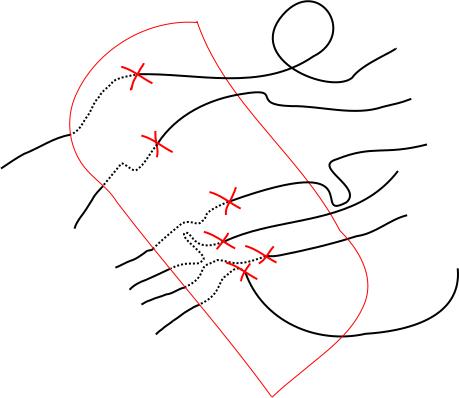
\includegraphics[width=0.55\textwidth]{Figures/PSOS.pdf}
  \end{center}

  Registriere Schnittpunkte von Trajektorie und \emph{Poincar\'e-Schnittebene}
\end{frame}


\begin{frame}{Billards: Übergang reguläre Dynamik $\to$ Chaos}

  Betrachte das Lima\c{c}on von Pascal: $r(\phi) = R + \epsilon\cos(\phi)$\\[0.5ex]
  $\leadsto$ \alert{Simulation}: Übergang reguläre Dynamik $\to$ Chaos\\[1ex]

  \only<2>{
    \begin{center}
      \includegraphics[width=0.85\textwidth]{Figures/Phasenraumbilder-crop.pdf}
  \end{center}}
\end{frame}


\begin{frame}{Konzept: der Lyapunov-Exponent}

  Wie sehr zwei benachbarte Trajektorien mit den Anfangsbedingungen $\vec\xi_0$ und $\vec\xi_0 + \delta\vec\xi_0$ auseinander laufen, kann quantifiziert werden:

  \begin{alertbbox}{Der Lyapunov-Exponent}
    Idee: eine kleine anfängliche  Störung $\delta\vec\xi_0$ wächst gemäß
    \[\abs{\delta\vec\xi(t)} = \eto{\lambda t}\abs{\delta\vec\xi_0}\,.\]
    Für jede Dimension des Systems gibt es einen Lyapunov-Exponenten $\lambda$.
  \end{alertbbox}
  \begin{itemize}
  \item $\lambda > 0$: exponentielles Auseinanderlaufen
  \item $\lambda < 0$: exponentielles Zusammenlaufen
  \item $\lambda = 0$: benachbart bleiben
  \end{itemize}
\end{frame}


\begin{frame}{Lyapunov-Exponent II}

  Eigenschaften:
  \begin{itemize}
  \item konservatives System: $\sum_i \lambda_i = 0$ (\emph{Satz von Liouville})
  \item dissipatives System: $\sum_i \lambda_i < 0$
  \end{itemize}

  \begin{exbox}{Berechnung des maximalen Lyapunov-Exponenten}
    \[\lambda = \lim\limits_{t\to\infty}\lim\limits_{\delta\vec\xi_0 \to \vec 0} \frac{1}{t}\ln\frac{\abs{\delta\vec\xi(t)}}{\abs{\delta\vec\xi_0}}\]
  \end{exbox}

  \begin{exbox}{Konzept: lokaler Lyapunov-Exponent}
    Expansion/Schrumpfung einer kleinen Kugel von Anfangsbedingungen um ein $\vec\xi_0$
    ist gegeben durch die Eigenwerte der Jacobi-Matrix $\partial\vec f/\partial \vec \xi\vert_{\vec\xi_0}$
    (mit $\vec f$ dem Fluß/der Abbildung).
  \end{exbox}
\end{frame}


\begin{frame}{Abhängigkeit von Anfangsbedingungen -- \emph{revisited}}

  Betrachte für das reguläre Lima\c{c}on mit $\epsilon=0.2$ einen kleinen Kreis von Anfangsbedingungen:

  \only<1>{
    \begin{center}
      \includegraphics[width=0.65\textwidth]{Figures/{Lim_eps0.2_iteration0}.png}
  \end{center}}

  \only<2>{
    \begin{center}
      \includegraphics[width=0.65\textwidth]{Figures/{Lim_eps0.2_iteration1}.png}
  \end{center}}

  \only<3>{
    \begin{center}
      \includegraphics[width=0.65\textwidth]{Figures/{Lim_eps0.2_iteration2}.png}
  \end{center}}

  \only<4>{
    \begin{center}
      \includegraphics[width=0.65\textwidth]{Figures/{Lim_eps0.2_iteration7}.png}
  \end{center}}

  \only<5>{
    \begin{center}
      \includegraphics[width=0.65\textwidth]{Figures/{Lim_eps0.2_iteration19}.png}
  \end{center}}

  \only<6>{
    \begin{center}
      \includegraphics[width=0.65\textwidth]{Figures/{Lim_eps0.2_iteration40}.png}
  \end{center}}

  \only<7>{
    \begin{center}
      \includegraphics[width=0.65\textwidth]{Figures/{Lim_eps0.2_iteration99}.png}
  \end{center}}
\end{frame}


\begin{frame}{Abhängigkeit von Anfangsbedingungen -- \emph{revisited}}

  Betrachte nun das chaotische Lima\c{c}on mit $\epsilon=0.45$ ebenfalls einen
  kleinen Kreis von Anfangsbedingungen:

  \only<1>{
    \begin{center}
      \includegraphics[width=0.65\textwidth]{Figures/{Lim_eps0.45_iteration0}.png}
  \end{center}}

  \only<2>{
    \begin{center}
      \includegraphics[width=0.65\textwidth]{Figures/{Lim_eps0.45_iteration1}.png}
  \end{center}}

  \only<3>{
    \begin{center}
      \includegraphics[width=0.65\textwidth]{Figures/{Lim_eps0.45_iteration4}.png}
  \end{center}}

  \only<4>{
    \begin{center}
      \includegraphics[width=0.65\textwidth]{Figures/{Lim_eps0.45_iteration6}.png}
  \end{center}}

  \only<5>{
    \begin{center}
      \includegraphics[width=0.65\textwidth]{Figures/{Lim_eps0.45_iteration9}.png}
  \end{center}}

  \only<6>{
    \begin{center}
      \includegraphics[width=0.65\textwidth]{Figures/{Lim_eps0.45_iteration11}.png}
  \end{center}}

  \only<7>{
    \begin{center}
      \includegraphics[width=0.65\textwidth]{Figures/{Lim_eps0.45_iteration15}.png}
  \end{center}}

  \only<8>{
    \begin{center}
      \includegraphics[width=0.65\textwidth]{Figures/{Lim_eps0.45_iteration19}.png}
    \end{center}

    $\leadsto$ \alert{mischende} Dynamik!
  }
\end{frame}

\section{Zusammenfassung}

\subsection{Zusammenfassung}

\begin{frame}{Zusammenfassung}

  Wir haben kennengelernt...

  \begin{itemize}
  \item \dots was \alert{Chaos} ist
  \item \dots wie sich Chaos konkret in einem dissipativen und einem konservativen System gestaltet
  \item \dots weshalb wir uns mit \alert{Billards} beschäftigen
  \item \dots wie ein \alert{Übergang} ins Chaos aussehen kann
  \end{itemize}

  Literatur:
  \begin{itemize}
  \item Alligood, Yorke, Sauer, \emph{Chaos}, Springer 1996
  \item T\'el, Gruiz, \emph{Chaotic Dynamics}, Cambridge 2006
  \end{itemize}

\end{frame}


\end{document}
